\section{Το πρόβλημα της πρόβλεψης ακολουθιών}

	Τα σύνορα της τεχνητής νοημοσύνης εκτείνονται πέρα από το παραδοσιακό πρόβλημα της εκμάθησης ενός στατικού συνόλου δεδομένων με επιβλεπόμενες μεθόδους,
	όπως γίνεται σε πολλές σύγχρονες εφαρμογές \parencite{lecun}.
	Η τεχνητή νοημοσύνη καλείται σήμερα να αξιοποιήσει τις καταιγιστικές ροές δεδομένων που παρέχει το (ανθρωπογενές και μη) περιβάλλον, σε πραγματικό χρόνο,
	και δίχως την πολυτέλεια της προσήμανσης που απαιτεί η επιβλεπόμενη μάθηση ---
	εφαρμογές IoT που απαιτούν δυναμική αλληλεπίδραση με το περιβάλλον τους έρχονται στο μυαλό \parencite{mohammadiDeepLearningIoT2018}.

	Επομένως, καλούμαστε να μοντελοποιήσουμε έναν κόσμο που αλλάζει \parencite{staticbottleneck}.
	Το μοντέλο οφείλει ή να είναι γενικότερο από όλες τις δυνατές μεταβολές του κόσμου ή να αλλάζει μαζί του.
	Η έννοια της ροής δεδομένων που αναφέρθηκε υπονοεί την έννοια του χρόνου, της αλληλουχίας, που επιτρέπει στο μοντέλο να αντλήσει πληροφορία από την αιτιώδη σχέση.
	Την ερμηνεία του κόσμου με τη βοήθεια της συνεπαγωγής και της αναγνώρισης απαιτήσεων και συνεπειών.

	Ορίζεται έτσι το πρόβλημα της εκμάθησης και πρόβλεψης ακολουθιών.
	Δηλαδή, ο πράκτορας που παρακολουθεί μια αλληλουχία δεδομένων (γεγονότων) καλείται να προβλέψει τη συνέχεια και να δράσει έτσι, ώστε βέλτιστα να ανταμειφθεί.
	Η ανταμοιβή, το κίνητρο και γενικότερα ο στόχος έχουν τεθεί από εξωτερικό παράγοντα και βρίσκονται εκτός του πλαισίου του προβλήματος.
	Άμεση εφαρμογή της πρόβλεψης είναι και η αναγνώριση ανωμαλιών.

	Η εκμάθηση ακολουθιών είναι κλασικό πρόβλημα, για το οποίο έχουν αναπτυχθεί κλασικές λύσεις.
	Κυριότερο και ευρύτερα διαδεδομένο είδος μοντέλων, ειδικά πριν τη σύγχρονη επάνοδο των νευρωνικών δικτύων, είναι τα Hidden Markov Models.
	Τα κλασικά νευρωνικά δίκτυα προσφέρουν στο πρόβλημα τα νευρωνικά δίκτυα χρονικής καθυστέρησης (TDNN).
	Η ουσιαστική συνεισφορά των κλασικών νευρωνικών δικτύων επιτυγχάνεται όμως με τα ανάδρομα δίκτυα (RNN),
	που γενίκευσαν τις παλαιότερες προσθιοδρομικές (feedforward) αρχιτεκτονικές ακριβώς για να μπορούν να αντιμετωπίσουν εγγενώς προβλήματα ακολουθιών.
	Ιδιαίτερης μνείας χρήζει η δομή «μακράς βραχυπρόθεσμης μνήμης» (LSTM).
	Από το 2015 έχει χρησιμοποιηθεί με επιτυχία σε ποικίλες εφαρμογές πολύ πιο σύνθετες από την εισαγωγή που παρουσιάζεται εδώ,
	όπως ως τεχνητή νοημοσύνη που παίζει το παιχνίδι StarCraft 2 \parencite[AlphaStar][]{vinyalsAlphaStarMasteringRealTime2019}.

	Σε αυτόν το χώρο λύσεων υπάρχουν παρόλα αυτά σημεία για βελτίωση.
	Οι περισσότερες εφαρμογές, συμπεριλαμβανομένου του AlphaStar, βασίζονται σε επιβλεπόμενη και ενισχυτική μάθηση,
	αφήνοντας ευρύ πεδίο εξερεύνησης για μη επιβλεπόμενα μοντέλα.
	Καθώς ο όγκος των ροών δεδομένων αυξάνεται εκθετικά \parencite{losingIncrementalOnlineLearning2018},
	παρατηρείται αυξανόμενη ζήτηση για αλγορίθμους που προσαρμόζονται γρήγορα στις εξελισσόμενες στατιστικές των δεδομένων τους (συνεχής μάθηση),
	έχοντας πρόσβαση μόνο σε μικρό χρονικό παράθυρο πληροφορίας.
	Στην προσπάθεια αυτή αναπτύσσονται ενεργά τεχνικές για βελτίωση της αποδοτικότητας δειγμάτων της μάθησης \parencite[όπως][]{nachumDataEfficientHierarchicalReinforcement2018},
	ή για παράκαμψη του προβλήματος, όπως η μεταφορική μάθηση (transfer learning) \parencite{xiongApplicationTransferLearning2018}.
	\medskip

	Στην ανάλυση των διαφόρων τρόπων ορισμού της τεχνητής νοημοσύνης, ο Wang \parencite{wangWhatYouMean2008} αναγνωρίζει τη μέθοδο
	«από τη δομή» για την έρευνα σε συστήματα που εμπνέονται ή μιμούνται
	το βασικό παράδειγμα ευφυούς συστήματος που επιλύει διαρκώς το παραπάνω πρόβλημα: τον εγκέφαλο, και ειδικά το φλοιό.
	Παρατηρείται μια τάση στο χώρο των τεχνητών νευρωνικών δικτύων ανασκόπησης της επαφής τους με τη βιολογική πραγματικότητα τα τελευταία χρόνια,
	όπως στο \cite{bengioBiologicallyPlausibleDeep2015}.
	Το πιο ηχηρό παράδειγμα είναι ο μηχανισμός κάψουλας που πρότειναν ο Hinton και συνεργάτες \parencite{sabourMatrixCapsulesEM2018,sabourDynamicRoutingCapsules2017}.
	\smallskip

	Σε αυτό λοιπόν το πλαίσιο, η μελέτη της HTM κρίνεται ιδιαίτερα καίρια.

\section{Στοιχεία της Hierarchical Temporal Memory}

Παρακάτω θα αναφερθούμε πάλι σε στοιχεία νευροεπιστήμης.
Καθώς ο σκοπός της περιγραφής είναι η κατανόηση των αλγορίθμων HTM, πρέπει να γίνει αποδεκτή μια παρέκκλιση από την αυστηρότητα, χάριν απλότητας.
Σε ό,τι βιολογικό στοιχείο αναφερθεί, ο αναγνώστης ας έχει υπόψιν ότι η πραγματικότητα είναι πάντα πιο πολύπλοκη και ότι αυτά που γράφονται εδώ δεν είναι ακριβώς ορθά.
Είναι, όμως, \textit{χρήσιμες προσεγγίσεις}.

Η κεντρική θέση στην οποία βασίζεται η Hierarchical Temporal Memory τμηματοποιεί τον εγκεφαλικό φλοιό σε ένα ψηφιδωτό βασικών μονάδων επεξεργασίας,
των \textbf{"φλοιικών στηλών" (cortical columns)},
που έχουν την ίδια δομή και εκτελούν τους \textbf{ίδιους αλγορίθμους, αλλά σε διαφορετικά δεδομένα}.
Η ιδέα αυτή έχει μακρά ιστορία στη νευροεπιστήμη, με μια συγκεντρωτική επισκόπηση από Defelipe, Markram κ.ά \cite{defelipeNeocorticalColumn2012}
να την οριοθετεί και να παρουσιάζει την ευρεία χρήση και κακομεταχείριση του όρου.
Για παράδειγμα, η εισαγωγική πρόταση περί "ψηφιδωτού" παραπάνω πρέπει να αντιμετωπιστεί μόνο ως πρώτη προσέγγιση,
γιατί οι στήλες δε φέρονται να εχουν γεωμετρικά σαφή σύνορα μεταξύ τους, αλλά διάχυτες ζώνες μετάβασης.
Πρεσβευτής και βασικός αποκρυσταλλωτής της ιδέας είναι ο Mountcastle \parencite{mountcastleColumnarOrganizationNeocortex1997},
με την ιδέα να χαίρει τόσο αποδοχής \parencite{haueisLifeCorticalColumn2016}, όσο και κριτικής ως προς τη χρησιμότητά της \parencite{hortonCorticalColumnStructure2005}.
Παρόλα αυτά, εδώ θα την υιοθετήσουμε.
Έτσι, ο εγκεφαλικός φλοιός αποδομείται σε πλειάδα μονάδων επεξεργασίας κοινής αρχής, και οι αλγόριθμοι που θα παρουσιαστούν περιγράφουν τη λειτουργία της μονάδας.

Η φλοιική στήλη είναι λοιπόν ένας πληθυσμός νευρώνων με κοινή συνδεσμολογία: λαμβάνουν το σήμα εισόδου από κοινές πηγές και στέλνουν το σήμα εξόδου σε κοινούς παραλήπτες.
Συχνά, τέτοιοι παραλήπτες είναι άλλες φλοιικές στήλες.
Συντάσσονται έτσι επεξεργαστικές \textbf{ιεραρχίες}, με τα πρώτα στάδια της ιεραρχίας να δημιουργούν απλούστερα μοντέλα για τον κόσμο από τα μετέπειτα
(κυρίως γιατί τα μετέπειτα συγκεντρώνουν περισσότερη πληροφορία).

Οι νευρώνες στους οποίους αναφερόμαστε παραπάνω, οι πυραμιδοειδείς νευρώνες, βρίσκονται κάθε στιγμή σε 1 από 2 καταστάσεις: ενεργοί ή ανενεργοί.
Η ενεργοποίησή τους ("δυναμικό δράσης") ερεθίζει άλλους νευρώνες με τους οποίους συνδέονται και μπορεί να τους οδηγήσει σε ενεργοποίηση.
Μπορούμε λοιπόν να περιγράψουμε την κατάσταση του φλοιού κάθε στιγμή ως το σύνολο των νευρώνων που είναι ενεργό.
Προκύπτει ότι το σύνολο αυτό είναι πολύ μικρό ποσοστό του συνολικού νευρικού πληθυσμού, δηλαδή η ενεργοποίηση είναι \textbf{αραιή}, περίπου 2\%.

Το μοτίβο ενεργοποίησης ενός πληθυσμού νευρώνων της ίδιας στήλης αποτελεί στο πλαίσιο της θεωρίας HTM τη δομή δεδομένων του εγκεφάλου
και ονομάζεται \textbf{αραιή διανεμημένη αναπαράσταση (SDR)}.
Κάθε αίσθηση στέλνει SDR στις στήλες που την επεξεργάζονται\char"0387  κάθε στήλη στέλνει SDR στους μύες ή σε άλλες στήλες ως έξοδο.
Η είσοδος σε ένα μοντέλο HTM πρέπει επομένως να μεταφράζει τη φυσική ποσότητα που θέλουμε να επεξεργαστούμε σε SDR, με τη διαδικασία να ονομάζεται \textbf{κωδικοποίηση}.
Αντίστοιχα, η ερμηνεία ενός SDR εξόδου ονομάζεται \textbf{αποκωδικοποίηση}.

Από τους κοινούς αλγορίθμους που υλοποιεί κάθε φλοιική στήλη, η HTM αυτή τη στιγμή περιγράφει 2: τη \textbf{χωρική συγκέντρωση} και τη \textbf{χρονική μνήμη}.
Η χρονική συγκέντρωση είναι επίσης διαδικασία που υποτίθεται, αλλά δεν έχει περιγραφεί επαρκώς και αποτελεί βασικό σημείο για περαιτέρω μελέτη.

\subsection{Αραιές Διανεμημένες Αναπαραστάσεις (SDR)}

Με βάση την παρατήρηση της αραιής πυροδότησης των νευρώνων στον εγκέφαλο σχεδιάζουμε ένα μεγάλο, αραιό, δυαδικό διάνυσμα που αναπαριστά την πυροδότηση ή μη κάθε νευρώνα της μελετούμενης περιοχής.
Μπορεί να θεωρηθεί ότι κάθε περιοχή ανταλλάσσει τέτοια μεγάλα αραιά δυαδικά διανύσματα με τις επόμενες.
Ουσιαστικά, αυτά τα αραιά διανύσματα αποτελούν τη ``δομή δεδομένων'' \cite{neuronssynapses,sdrkanerva} του εγκεφάλου.
Το ιδιαίτερο χαρακτηριστικό αυτών των διανυσμάτων, λόγω αυτού που αναπαριστούν, είναι ότι κάθε ξεχωριστό bit τους φέρει σημασιολογικό νόημα -- αντίθετα δηλαδή από την κωδικοποίηση ενός γράμματος σε κώδικα ASCII, όπου νόημα φέρει μόνο η πλήρης ``λέξη''.
Εξού και το ``distributed'' του ονόματος.

\subsubsection{Χωρητικότητα SDR}

Η χωρητικότητα ενός SDR με μέγεθος n και cardinality (πλήθος μονάδων) w είναι το πλήθος των διαφορετικών SDR με αυτή τη μορφή, δηλαδή οι συνδυασμοί των n ανά w: $$ \binom nw= \frac{n!}{w!(n-w)!} $$

\subsubsection{Συνδυασμοί SDR}
Διαφάνεια 9.

\subsubsection{Σύνολα SDR}

Διαφάνεια 10.

Επισημαίνεται μονάχα η \emph{σχεδιαστική ελευθερία} που παρέχουν τα SDR.
Όσο μεγαλύτερα SDR χρησιμοποιούνται, τόσο αυξάνεται ο χώρος των ενδεχομένων και τόσο πιο απίθανα γίνονται τα λανθασμένα ταιριάσματα.


\subsection{Μοντέλο νευρώνα}

Πρώτα απ'όλα: νευρώνα ονομάζουμε μια δομή που δέχεται σήματα από άλλους νευρώνες και, όταν αυτά πληρούν κάποιες προϋποθέσεις, ενεργοποιείται, για να στείλει σήματα στους επόμενους νευρώνες.
Η επαφή 2 νευρώνων καλείται σύναψη.

Ο βιολογικός νευρώνας (συγκεκριμένα πυραμιδοειδής νευρώνας που απαντά συχνά στο neocortex) είναι ένα σύνθετο στοιχείο, με πολλούς χώρους και διανεμημένες λειτουργίες, που υλοποιούν τις λογικές πράξεις της άθροισης, του πολλαπλασιασμού, της χωρικής και χρονικής ολοκλήρωσης ταυτόχρονα και παράλληλα σε διαφορετικές ομάδες εισόδων.
Η κεντρική δομή του νευρώνα, το σώμα, δέχεται ερεθίσματα από το προηγούμενο ιεραρχικά επίπεδο.
Αν έρθουν αρκετά τέτοια ερεθίσματα σε σύντομο χρονικό διάστημα ο νευρώνας ενεργοποιείται.
Οι πηγές των σημάτων που ο νευρώνας λαμβάνει στο σώμα του ονομάζονται \emph{receptive field} του νευρώνα.
Περιφερειακά του σώματος υπάρχουν τα δενδριτικά τμήματα, στα οποία υπάρχουν συνάψεις με νευρώνες του ίδιου επιπέδου, που παρέχουν την πληροφορία των συμφραζόμενων.
Κάθε τμήμα αυτόνομα δέχεται σήματα και, αν αυτά είναι αρκετά, προκαλείται ένα NMDA spike.
Σε αντίθεση με την ενεργοποίηση του σώματος, αυτό γενικά δεν αρκεί για να ενεργοποιήσει ολόκληρο το νευρώνα· θέτει όμως το νευρώνα σε κατάσταση ``επιφυλακής'', διευκολύνοντας τη μετέπειτα ενεργοποίησή του από σωματικά ερεθίσματα.
Ο νευρώνας επίσης λαμβάνει ερεθίσματα από την πλευρά του άξονα, από τους νευρώνες δηλαδή που ``δέχονται'' το σήμα του στην κανονική του πορεία.
Αυτά αποτελούν σήματα ανάδρασης.

Μια απλοποιημένη εκδοχή αυτής της περιγραφής αποτελεί και ο υπολογιστικός νευρώνας του συστήματος που επιδεικνύεται.
Έχει πάλι 3 περιοχές που συμπεριφέρονται διαφορετικά για να λαμβάνει εισόδους feedforward, context και feedback όπως ο βιολογικός.
Επαρκής feedforward είσοδος αρκεί για να τον ενεργοποιήσει, ενώ επαρκής είσοδος context ή feedback τον θέτει στο λεγόμενο ``predictive state''.
Αν στη συνέχεια (στη συνέχεια...
ακολουθία...
συνεπαγωγή...) έρθει feedforward είσοδος, θα ενεργοποιηθεί πιο εύκολα και γρήγορα απ'ό,τι άλλοι νευρώνες με την ίδια είσοδο.
Σε αντιπαραβολή, ο ``νευρώνας'' ενός κλασικού τεχνητού νευρωνικού δικτύου δεν έχει διακριτά λειτουργικά τμήματα και απλώς αθροίζει όλες τις εισόδους του.


\subsection{Μοντέλο δικτύου}

Και μόνο ο παραπάνω ανάδρομος ορισμός του νευρώνα παραπέμπει στο ρόλο του ως μονάδα δικτύου.

Η πρώτη οργανωτική δομή νευρώνων, τόσο στο neocortex, όσο και στο HTM, είναι το minicolumn.
Συνοπτικά, ο ρόλος των minicolumns είναι να επιτρέπουν διαφορετικές εσωτερικές αναπαραστάσεις των εξωτερικών (feedforward) ερεθισμάτων, ανάλογα με τα συμφραζόμενα.
Όλοι οι νευρώνες του minicolumn μοιράζονται \emph{το ίδιο receptive field}, ενώ μεταξύ τους υπάρχει \emph{inhibition}.
Έτσι υλοποιείται μια αρχιτεκτονική ``winner-takes-all'', όπου, αν κάποιοι νευρώνες είναι ήδη σε predictive κατάσταση όταν έρθει feedforward είσοδος που ερεθίζει το minicolumn, θα ενεργοποιηθούν πρώτοι και θα αποτρέψουν την ενεργοποίηση των υπολοίπων.
Η παραπάνω περιγραφή βέβαια προτρέχει λίγο.

Πολλά minicolumns συνθέτουν ένα cortical layer, που αποτελεί τη λειτουργική μονάδα ενός συστήματος HTM.
Κάθε minicolumn του cortical layer έχει διαφορετικές feedforward συνδέσεις προς την είσοδο του layer, ενώ διαφορετικά minicolumns μοιράζονται μεταξύ τους συνδέσεις που φέρουν πληροφορίες συμφραζομένων.
Σε πολλές περιπτώσεις μπορεί να υπάρχει ολικό inhibition μεταξύ των minicolumns.
Αν βέβαια το cortical layer έχει κάποια τοπολογική διάταξη προς την είσοδό του\footnote{Δες το βίντεο ``Topology (Episode 10)'' της σειράς ``HTM School'' \cite{htmschool}}, όπως συχνά συμβαίνει στον εγκεφαλικό φλοιό, τότε οι inhibitory συνδέσεις είναι τοπικές και ένα minicolumn δεν ανταγωνίζεται κάποιο άλλο που βρίσκεται μακριά του.
Τα λειτουργκά παραδείγματα παρακάτω αποτελούνται από 1 cortical layer.
Ένα πιο σύνθετο σύστημα θα μπορούσε να ενώσει εν σειρά πολλά cortical layers.

Οι συνάψεις των HTM νευρώνων είναι επίσης πιστότερες στη βιολογία.
Δε χρησιμοποιούν κάποιο βάρος που πολλαπλασιάζει την είσοδο, αλλά είναι δισταθείς, δηλαδή υπάρχουν ή όχι.
Ένα μέγεθος όμως που χαρακτηρίζει κάθε σύναψη είναι η \emph{μονιμότητά} της, που διαμορφώνεται δυναμικά από τη μαθησιακή διαδικασία (στην οποία δε θα αναφερθούμε παραπάνω εδώ) με αλγόριθμο τύπου Spike Timing Dependent Plasticity (STDP), που μπορεί ουσιαστικά να εμφανίσει και να εξαφανίσει υποθάλπουσες συνάψεις για να προσαρμόσει το σύστημα στα δεδομένα.
Η μονιμότητα μιας σύναψης συγκρίνεται με ένα κατώφλι και, αν είναι πιο πάνω είναι ενεργή, αν είναι πιο κάτω είναι ανενεργή.
Μια σύναψη με μονιμότητα λίγο πάνω από το κατώφλι μπορεί δηλαδή να απενεργοποιηθεί εύκολα.


\subsection{Encoders}

Ο εγκέφαλος έχει ως βασική διεπαφή με τον έξω κόσμο τον αμφιβληστροειδή χιτώνα του ματιού και τον κοχλία του αυτιού.
Και τα 2 αυτά συστήματα μπορούμε να θεωρήσουμε ότι μετατρέπουν τα φυσικά ερεθίσματα του κόσμου σε μια πρώτη μορφή SDR, για να ερεθίσουν με τη σειρά τους το επόμενο επίπεδο νευρώνων.
Το ρόλο αυτό στα συστήματα HTM καλύπτουν οι encoders.

Οι encoders μπορεί να είναι από πολύ απλά έως εξαιρετικά πολύπλοκα συστήματα (βλέπε αμφιβληστροειδή).
Στη διαφάνεια 13 δίνεται το παράδειγμα ενός απλού encoder που κωδικοποιεί ακέραιους αριθμούς συγκεκριμένου εύρους.
Μπορεί όμως να σχεδιαστεί και encoder που να κωδικοποιεί λέξεις ή και κείμενα, όπως κάνει η εταιρία cortical.io \cite{semantic} στη διαφάνεια 14.


\subsection{Decoders}


\section{Βασικές λειτουργίες HTM}

Παρουσιάζονται ένα σύστημα που κανονικοποιεί τα SDR εισόδου, ο \emph{Spatial Pooler}, και ένα σύστημα που μαθαίνει να αναγνωρίζει ακολουθίες απλών ερεθισμάτων, δηλαδή μια \emph{μνήμη ακολουθιών}.
Για το πρώτο προτείνονται τα σχετικά βίντεο από τη σειρά ``HTM School'' στο youtube, ενώ για το δεύτερο η αναφορά [2].
Λίγα λόγια για τη μνήμη ακολουθιών:

\subsection{Sequence Memory}

Στη \emph{διαφάνεια 17} \cite{continuous} βλέπουμε ένα cortical layer που αποτελείται από από minicolumns.
Στη μέση (C) βλέπουμε πώς αντιδρά το σύστημα καθώς δέχεται για πρώτη φορά τις αλληλουχίες ``ABCD'' και ``XBCY''.
Παρατηρούμε ότι κάθε σύμβολο εισόδου ενεργοποιεί συγκεκριμένα minicolumns (αυτά που διεγείρονται περισσότερο), και ότι σε κάθε τέτοιο minicolumn ενεργοποιούνται \emph{όλοι} οι νευρώνες.

Ας επικεντρωθούμε στο τι συμβαίνει όταν λαμβάνεται η είσοδος ``A''.
Ενεργοποιούνται τα minicolumns που φαίνονται, αλλά κάποιοι από τους ενεργοποιημένους νευρώνες έχουν context συνάψεις (ενεργές ή μη) με κάποιους νευρώνες που ενεργοποιεί η είσοδος ``B''.
Αυτό φαίνεται στη διαφάνεια 18 Α.
Αφού το σύστημα δει την αλληλουχία A -> B μερικές φορές, συνάψεις αυτού του τύπου ενεργοποιούνται μέσω της διαδικασίας εκμάθησης, ακόμα κι αν στην αρχή ήταν ανενεργές.
Έτσι, όταν ξαναέρθει η είσοδος ``A'', συγκεκριμένοι νευρώνες των στηλών που αντιστοιχούν στο ``B'' τίθενται σε predictive state.
Όταν λοιπόν όντως έρχεται η είσοδος ``B'' αμέσως μετά αυτοί οι νευρώνες ενεργοποιούνται πρώτοι και μπλοκάρουν μέσω inhibitory συνδέσεων τους υπόλοιπους του ιδίου minicolumn.
Έτσι καταλήγουμε στην ακολουθία της κάτω σειράς (D) της διαφάνειας 17.
Τα παραπάνω σημαίνουν ότι το σύστημα \emph{προβλέπει την επόμενη είσοδό του}, που είναι ο βασικός στόχος του προβλήματος εκμάθησης ακολουθιών.

Ο μηχανισμός αυτός οδηγεί σε δύο παρατηρήσεις: η εσωτερική αναπαράσταση κάθε συμβόλου είναι \emph{διαφορετική ανάλογα με τα συμφραζόμενα} και το σύστημα μπορεί να πραγματοποιεί \emph{πολλαπλές προβλέψεις ταυτόχρονα}.

Το πρώτο φαίνεται στην κάτω σειρά (D) από τους διαφορετικούς νευρώνες που ενεργοποιούνται για να συμβολίσουν την ίδια είσοδο ``B'', ανάλογα αν το προηγούμενο σύμβολο ήταν ``A'' ή ``X'', οπότε προκύπτει η εσωτερική αναπαράσταση B' ή B'' αντίστοιχα.
Το δεύτερο σημείο φαίνεται στη διαφάνεια 18 Β, όπου δίνεται η είσοδος ``B'', χωρίς να έχει προηγηθεί ``Α'' ή ``Χ''.
Το σύστημα τότε προβλέπει την ένωση των 2 καταστάσεων C' και C'', οι οποίες ενεργοποιούνται παράλληλα όταν όντως έρχεται η είσοδος C.
Εκείνη τη στιγμή λοιπόν το σύστημα σωστά προβλέπει ότι η συνέχεια της ακολουθίας θα είναι ή ``D'' ή ``Y''.

\section{Αποτελέσματα - Προσομοιώσεις}

To ΗΤΜ δοκιμάστηκε τόσο σε τεχνητά, όσο και σε πραγματικά δεδομένα για να αξιολογηθεί η δυνατότητα του να παρέχει ακριβείς προβλέψεις.
Παρακάτω θα αναλυθούν δύο παραδείγματα και θα δοθούν τα συγκριτικά διαγράμματα των επιδόσεων με άλλα νευρωνικά δίκτυα.

\subsubsection{Πρόβλεψη συμβόλου ακολουθίας}

Οι αλγόριθμοι του Hierarchical Temporal Memory (HTM) δοκιμάστηκαν σε διαφορετικά προβλήματα \cite{continuous,nab}, ώστε να αξιολογηθεί η επίδοση του συστήματος σε σχέση με άλλες υλοποιήσεις.
Στο πρώτο παράδειγμα έχουν δημιουργηθεί δύο ακολουθίες από σύμβολα, σύμφωνα με την εικόνα \eqref{fig:sequences}.
Στόχος είναι η πρόβλεψη του τελευταίου συμβόλου.
\begin{figure}[H]
	\centering%
	{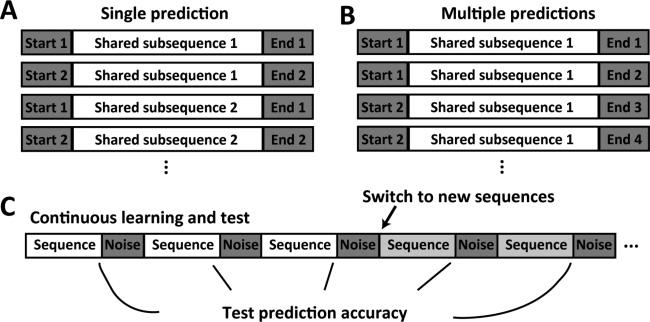
\includegraphics[width=0.8\columnwidth,clip=true]{figures/vlsi/sequences.jpg}}
	\caption{Ακολουθίες συμβόλων για την προσομοίωση} \label{fig:sequences}
\end{figure}

Οι ακολουθίες φτιάχτηκαν έτσι ώστε να χρειάζεται ένα βάθος μνήμης τουλάχιστον 2 παρελθοντικών συμβόλων για την επιτυχή πρόβλεψη.
Το πρώτο set ακολουθιών έχει δημιουργηθεί για να ελεγχθεί η δυνατότητα απλής πρόβλεψης, καθώς κάθε ακολουθία προσδιορίζεται πλήρως από τα πεδία ``Start'' και ``Shared Subsequence''.
Αντιθέτως, στο δεύτερο set δύο ακολουθίες μπορεί να έχουν ίδια τα παραπάνω πεδία.
Σε αυτή την περίπτωση το νευρωνικό δίκτυο θα πρέπει να επιτύχει την ορθή πρόβλεψη όλων των πιθανών καταλήξεων, δηλαδή την ταυτόχρονη πολλαπλή πρόβλεψη.
Τέλος, ανάμεσα στις ακολουθίες προστέθηκε ένα σύμβολο θορύβου, ώστε να εξεταστεί η ανθεκτικότητα του συστήματος σε αυτόν.
\begin{figure}[H]
	\centering%
	{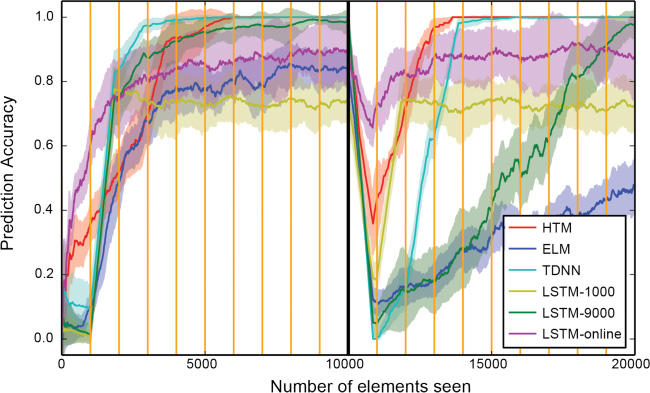
\includegraphics[width=0.7\columnwidth,clip=true]{figures/vlsi/single_prediction.jpg}}
	\caption{Απόδοση διαφορετικών υλοποιήσεων για απλή πρόβλεψη} \label{fig:single-prediction}
\end{figure}

Στο σχήμα \eqref{fig:single-prediction} δίνεται η συγκριτική απόδοση των διαφορετικών υλοποιήσεων νευρωνικών δικτύων για το πρώτο set ακολουθιών.
Τα δίκτυα που υλοποιούνται είναι το HTM, το ELM, το TDNN και το LSTM.
Ο προσδιορισμός στο LSTM αφορά το πλήθος των δειγμάτων που χρησιμοποιούνται για retraining σε κάθε κατακόρυφη κίτρινη γραμμή του διαγράμματος.
Στο στοιχείο 10000 που σημειώνεται με κάθετη κατακόρυφη γραμμή, αλλάζουν αμοιβαία τα δύο τελευταία σύμβολα κάθε ακολουθίας και μελετάται η προσαρμογή του δικτύου στο νέο input space.
Βλέπουμε ότι το HTM πετυχαίνει αρχικά σε έναν ικανοποιητικό αριθμό δειγμάτων ακρίβεια $100\%$.
Το πιο σημαντικό είναι, βέβαια, ότι μέσω online training αναπροσαρμόζεται ταχύτερα από κάθε άλλη υλοποίηση στο νέο χώρο ακολουθιών εισόδου.\\
\begin{figure}[H]
	\centering%
	{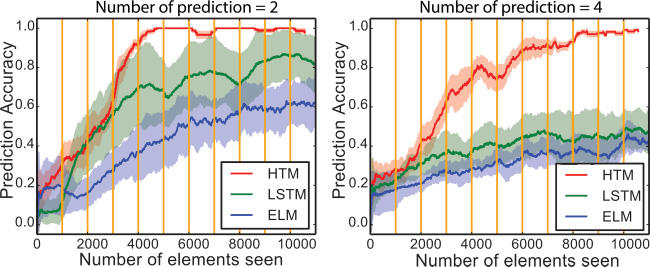
\includegraphics[width=0.8\columnwidth,clip=true]{figures/vlsi/multiple_predictions.jpg}}
	\caption{Απόδοση δικτύων για πολλαπλές προβλέψεις} \label{fig:multiple-prediction}
\end{figure}

Οι πολλαπλές προβλέψεις εξετάζονται από το δεύτερο σετ και τα συγκριτικά αποτελέσματα για διπλή και τετραπλή πρόβλεψη δίνεται στο σχήμα \eqref{fig:multiple-prediction}.
Όπως φαίνεται, το HTM είναι το μοναδικό σύστημα που πετυχαίνει μετά από κάποιο διάστημα ακρίβεια σχεδόν $100\%$.
Αυτό απορρέει από την αναπαράσταση μέσω SDR και τη δυνατότητα του Temporal Pooler για πολλαπλές προβλέψεις.\\
Στη συνέχεια, μελετήθηκε η απόδοση του HTM για ακολουθίες διαφορετικού μήκους.
Ένα από τα τα σημαντικότερα στοιχεία του Temporal Pooler είναι η δυνατότητα αναπροσαρμογής online του «βάθους» μνήμης που χρησιμοποιείται για την πρόβλεψη.
Έτσι, όπως παρατηρούμε και στο διάγραμμα \eqref{fig:sequence-order}, πετυχαίνει πρόβλεψη ακόμα και τάξης 100, που σημαίνει ότι απαιτείται μνήμη 99 συμβόλων για να προβλεφθεί επιτυχώς το τελευταίο.
Το πλήθος των ακολουθιών που απαιτείται για να εκπαιδευτεί το σύστημα και να πετύχει ακρίβεια κοντά στο $100\%$ αυξάνει γραμμικά με την τάξη της ακολουθίας.
\begin{figure}[H]
	\centering%
	{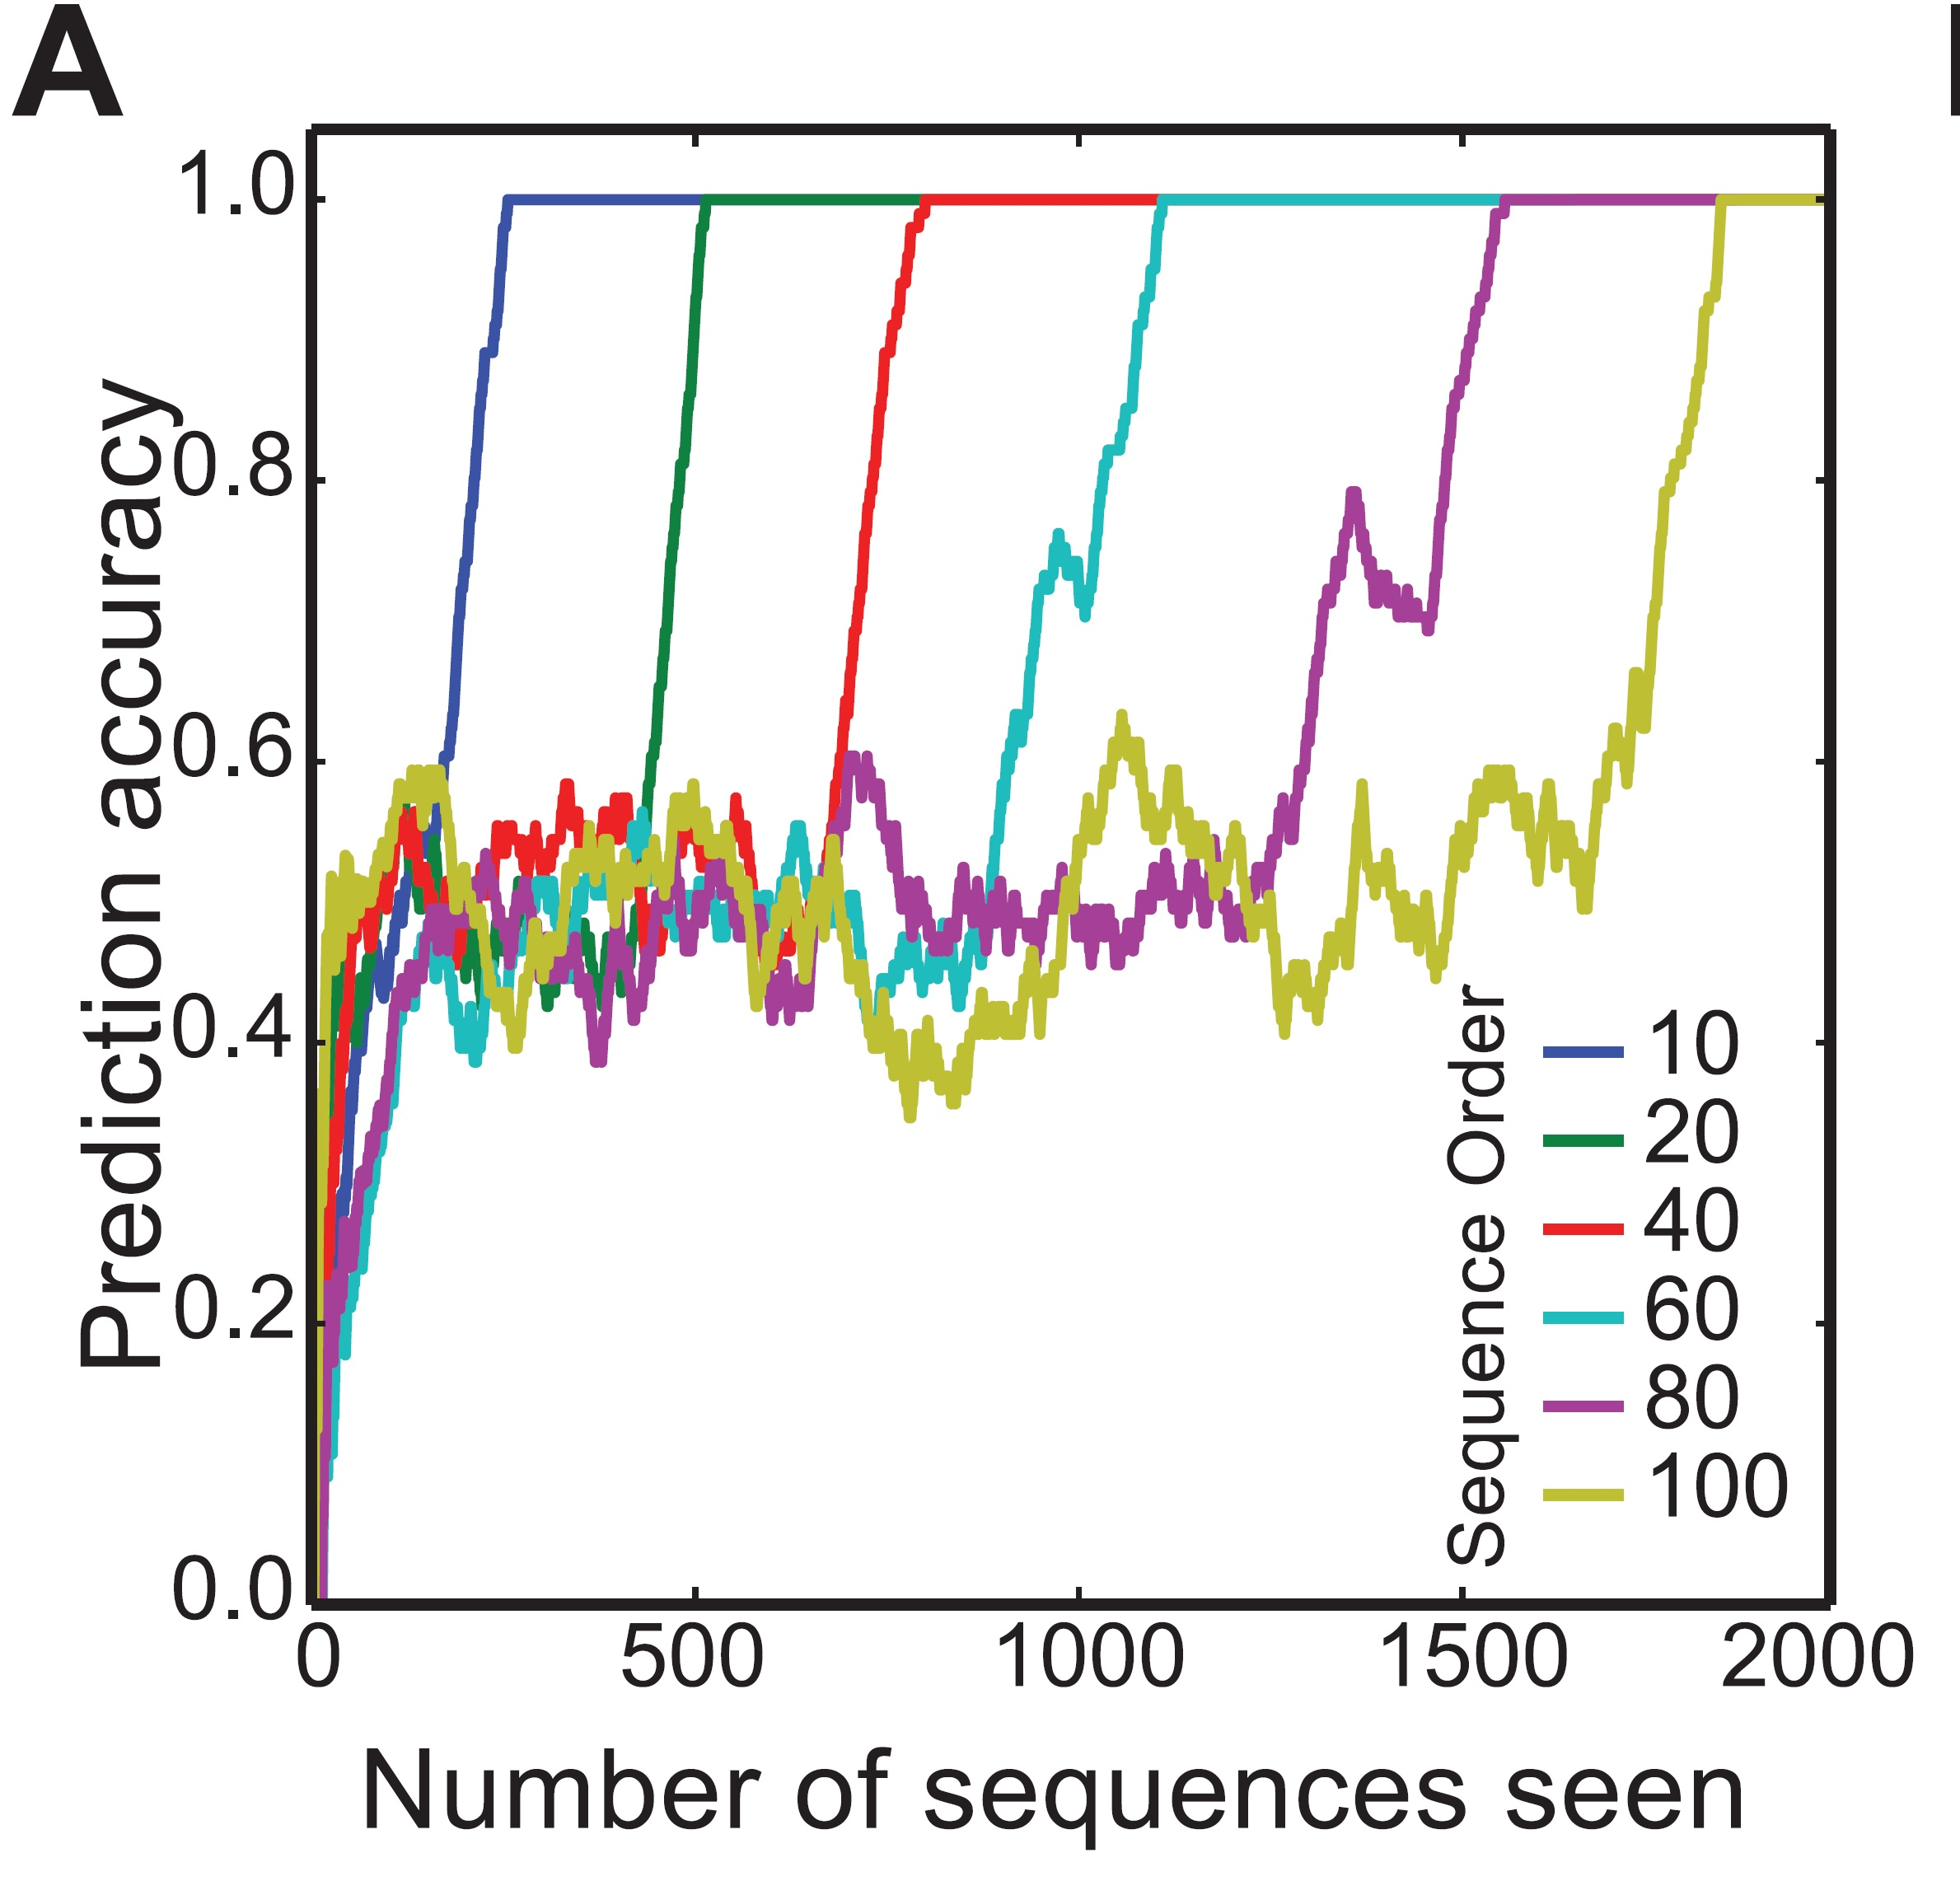
\includegraphics[width=0.4\columnwidth,clip=true]{figures/vlsi/sequence_order.jpg}}
	\caption{Απόδοση HTM συναρτήσει της τάξης της ακολουθίας} \label{fig:sequence-order}
\end{figure}

Τέλος, τα διαφορετικά συστήματα εξετάστηκαν και ως προς την ανθεκτικότητα σε καταστροφή του δικτύου μέσω νεκρών νευρώνων.
Το HTM έμεινε ανεπηρέαστο ακόμα για $30\%$ νεκρούς νευρώνες, συνθήκες κατά τις οποίες το ELM και το LSTM είχαν υποβαθμιστεί αρκετά.

\begin{figure}[H]
	\centering%
	{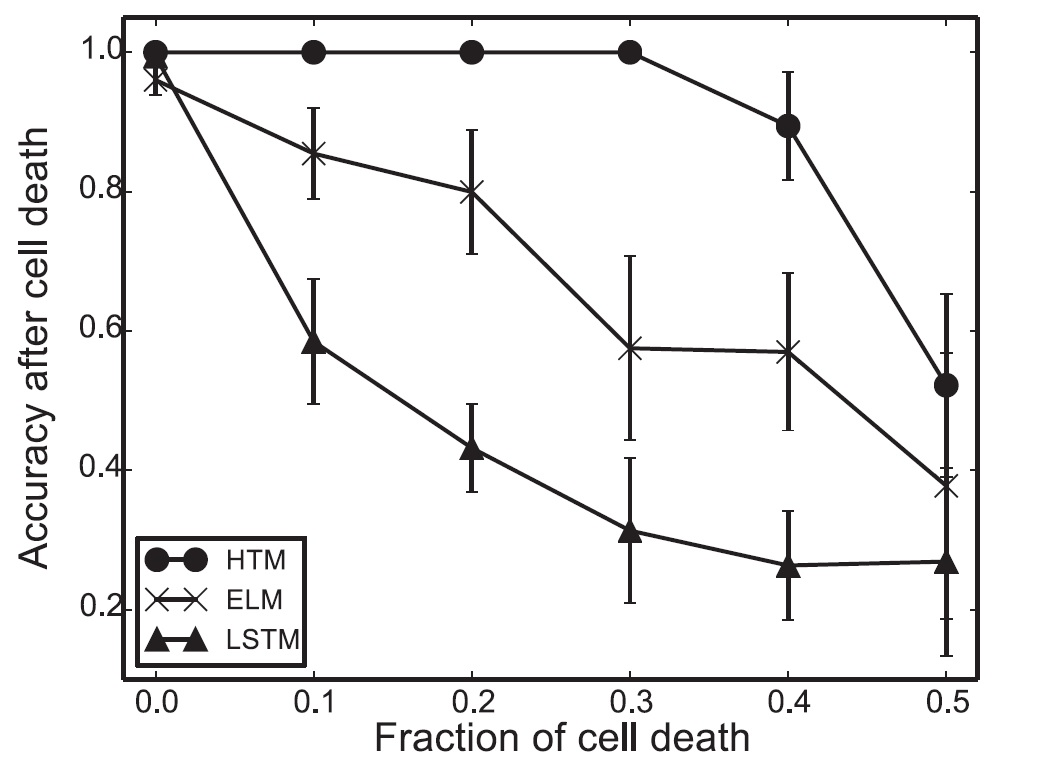
\includegraphics[width=0.4\columnwidth,clip=true]{figures/vlsi/cell_death.jpg}}
	\caption{Ανθεκτικότητα υλοποιήσεων σε νεκρούς νευρώνες} \label{fig:cell-death}
\end{figure}


\subsubsection{Πρόβλεψη της ζήτησης taxi στη Νέα Υόρκη}

Το Hierarchical Temporal Memory δοκιμάστηκε και σε πραγματικά streaming δεδομένα.
Πιο συγκεκριμένα, ζητήθηκε η πρόβλεψη της ζήτησης στα taxi της Νέας Υόρκης 2.5 ώρες πριν την πραγματική μέτρηση.
Η ζήτηση ποσοτικοποιήθηκε ως η συνολική εξυπηρέτηση πελατών σε ένα χρονικό παράθυρο 30 λεπτών.
Εξετάστηκαν διάφοροι τύποι νευρωνικών δικτύων, καθώς και το στατιστικό μοντέλο ARIMA.
%Όπως παρατηρούμε από την εικόνα \ref{fig:taxi_accuracy}, το HTM πέτυχε το μικρότερο απόλυτο σφάλμα πρόβλεψης (της τάξης του $0.08\%$ ).\\

\begin{figure} [H]
	\centering%
	\begin{subfigure}{0.5\columnwidth}
		{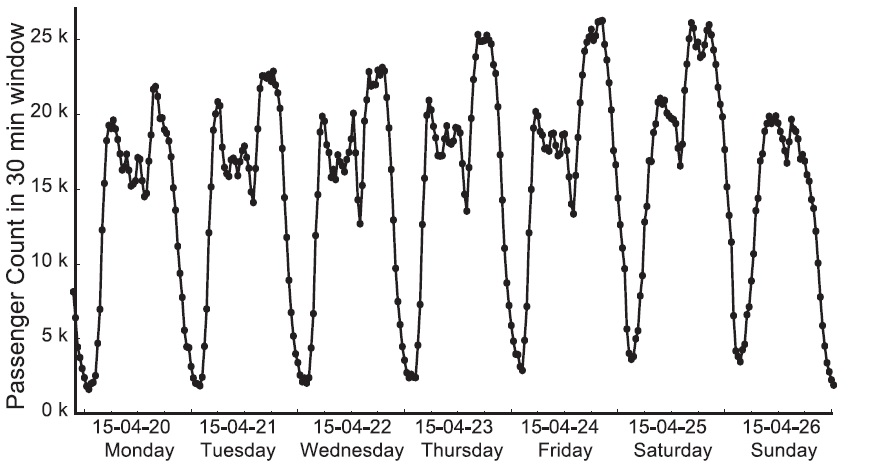
\includegraphics[width=\columnwidth,clip=true]{figures/vlsi/taxi_demand.jpg}}
		\caption{Διάγραμμα ζήτησης}
		\label{fig:taxi_demand}
	\end{subfigure}%
	\begin{subfigure}{0.5\columnwidth}
		\centering
		{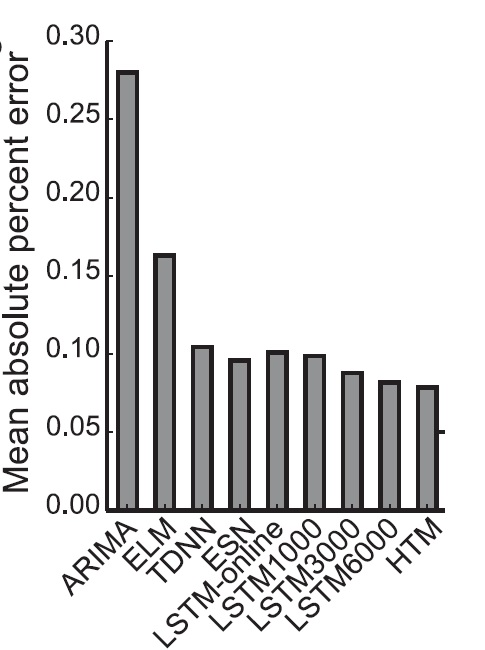
\includegraphics[width=0.5\columnwidth,clip=true]{figures/vlsi/taxi_accuracy.jpg}}
		\caption{Μέσο απόλυτο σφάλμα}
		\label{fig:taxi_accuracy}
	\end{subfigure}
	\caption{Πρόβλεψη ζήτησης των taxi}
	\label{fig:taxi_simulation}
\end{figure}

Στη συνέχεια, τα δεδομένα εισόδου τροποποιήθηκαν τεχνητά ανεβάζοντας ή μειώνοντας τη ζήτηση κατά $20\%$ σε διαφορετικές χρονικές περιόδους εντός κάθε μέρας.
Στόχος ήταν να μελετηθεί η προσαρμογή του δικτύου στις νέες (τεχνητές) συνήθειες των επιβατών taxi της Νέας Υόρκης.
Η αλλαγή πραγματοποιήθηκε την 1η Απριλίου και εντός 2 βδομάδων το σύστημα HTM αναπροσάρμοσε το μοντέλο του, ώστε να πετυχαίνει εκ νέου σωστές προβλέψεις.
Σε αντίθεση, το LSTM είτε απέτυχε να επανέρθει, είτε χρειάστηκε πολύ περισσότερο διάστημα για retraining των παραμέτρων του.

\begin{figure}[h]
	\centering%
	{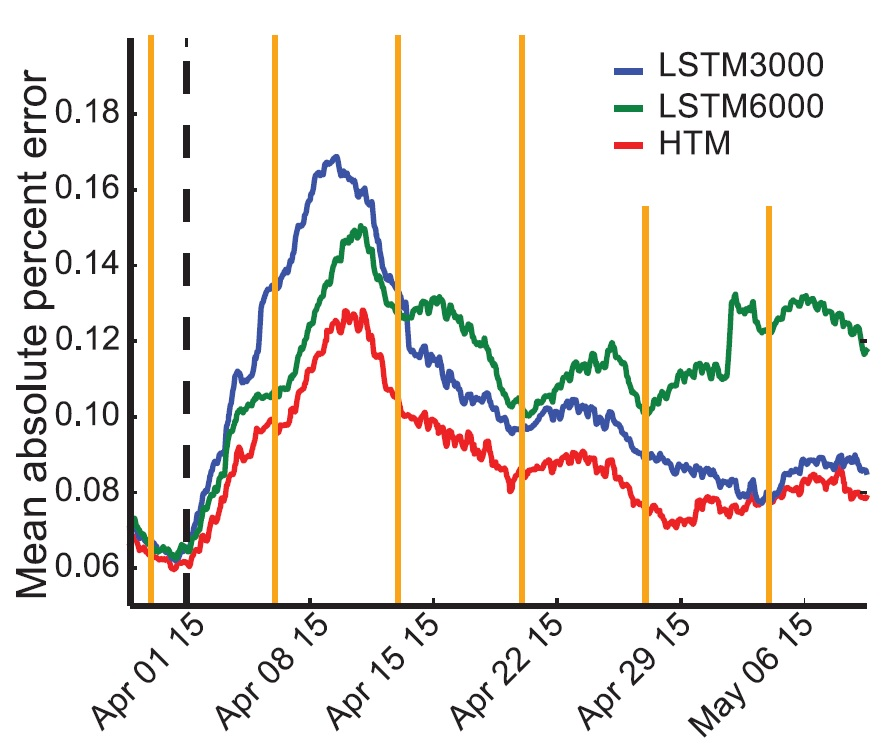
\includegraphics[width=0.4\columnwidth,clip=true]{figures/vlsi/taxi_adaptation.jpg}}
	\caption{Προσαρμογή δικτύων σε μεταβολή της ζήτησης}
	\label{fig:taxi-adaptation}
\end{figure}
